Debido a que tenemos un dataset con un número tan grande de datos, para poder enfrentarnos a un problema de clasificación hemos decidido quedarnos con las muestras del dataset relativas a avistamientos de 5 especies de pokemon (Exeggcute, Squirtle, Pinsir, Meowth y Kakuna). No hemos optado por quedarnos con muestras relativas a 5 tipos de pokemon ya que, por un lado el número de datos seguiría siendo demasiado grande para tratarlo computacionalmete, y por otro consideramos que los datos relativos a las muestras de una especie de pokemon serían más homogéneos que aquellos relativos a un tipo de pokemon concreto. Optamos por estas especies ya que tienen un número adecuado de muestras y no están demasiado desequilibradas, aunque como veremo más adelante estas medidas no han sido especialmente efectivas de cara a los resultados de la clasificación.\\

Una vez hemos elegido el subconjunto de datos sobre el que trabajaremos vamos a realizar un proceso de preprocesamiento sobre este conjunto para poder hacerlo operativo de cara a los métodos de clasificación que emplearemos. Así, en primer lugar eliminamos los atributos \textbf{pokemonId} y \textbf{class} ya que esta información es justamente la que intentamos predecir con los distintos algoritmos que probaremos. Por otro lado también eliminamos el \textbf{tipo} del pokemon; este tipo se deduce directamente de la clase del pokemon con lo que no obtendríamos unos resultados de clasificación reales si lo dejásemos en el nuevo dataset.\\

A continuación limpiamos el dataset eliminando aquellos atributos que sólo presenten un valor a lo largo de todas las muestras, estos atributos no aportarán ninguna información al proceso de clasificación.\\

En un primer uso del dataset para probar los árboles de decisión nos encontramos con que una variable factor tenía más de 32 niveles con lo que los árboles no podían trabajar con nuestro dataset. Al revisar los tipos de variable del dataset nos encontramos con la el atributo \textbf{pokestopDistanceKm} era de tipo factor. Esto no tiene sentido ya que realmente esta variable es simplemente una variable que nos da la distancia en kilómetros del avistamiento de un pokemon a una poke-parada. Por lo tanto pasamos esta variable a numérica.\\

Al pasar esta variable a numérica observmos que teníamos valores perdidos en nuestro dataset, algo que se nos había pasado por alto anteriomente. Pasamos entonces a revisar si nuestro dataset buscando valores perdido, dado que sólo teníamos una muestra que presentase un valor perdido decidimos eliminarla del dataset simplemente.\\

Además, dado a que vamos a hacer uso de algoritmos como el KNN que dependen de la distancia entre las distintas muestras, antes de pasar a emplear estos algoritmos vamos a realizar una normalización de las variables al intervalo [0,1]. Por esta misma razón pasamos aquellos atributos categóricos de dos niveles (que son 1 y 2) a variables numéricas con valores 0 y 1. Estros atributos son los relativos a las coocurrencias y el \textbf{closeToWater}.\\

Nuevamente debido a la influencia de la distancia pasamos los atributos categóricos con más de 2 niveles  a atributos binarios, uno por cada nivel de cada uno de estos atributos. Por otro lado al intentar usar la función tree para obtener un árbol de decisión obtuvimos un error diciendo que teníamos una variable categórica con más de 32 nivels, observamos que el atributo \textbf{pokestopDistanceKm} era categórico, algo que no consideramos que tenga mucho sentido. Con lo cual pasamos a transformar este atributo a numérico. 

Con el dataset con esta configuración pasamos a aplicar y probar diversos algoritmos de clasificación sobre nuestro dataset. Para ello elaboramos una partición de train y otra de test (80-20) empleando la función \code{createDataPartition} del paquete \code{caret} que tiene la ventaja de que elabora estas particiones manteniendo la proporción entre las distintas especies del dataset. Obtuvimos así los siguientes resultados:

\begin{table}[H]
\centering
\caption{Resultados de clasificación}
\label{my-label}
\begin{tabular}{|l|c|}
\hline
\rowcolor[HTML]{FFFC9E} 
\multicolumn{1}{|c|}{\cellcolor[HTML]{FFFC9E}\textbf{Algoritmo}} & \textbf{Tasa de acierto en test} \\ \hline
tree                                                             & 34.12\%                          \\ \hline
ctree                                                            & 39.53\%                          \\ \hline
rpart                                                            & 38.43\%                          \\ \hline
KNN (k = 9)                                                      & 34.12\%                          \\ \hline
random forest                                                    & 44.75\%                          \\ \hline
xgboost                                                          & 45.90\%                          \\ \hline
\end{tabular}
\end{table}

En primer lugar hemos empleado árboles de decisión, en concreto hemos probado 3 algoritmos distintos para construir árboles de decisión, el que mejor resultado a obtenido ha sido \textbf{ctree}.

\begin{figure}[H]
	\centering
	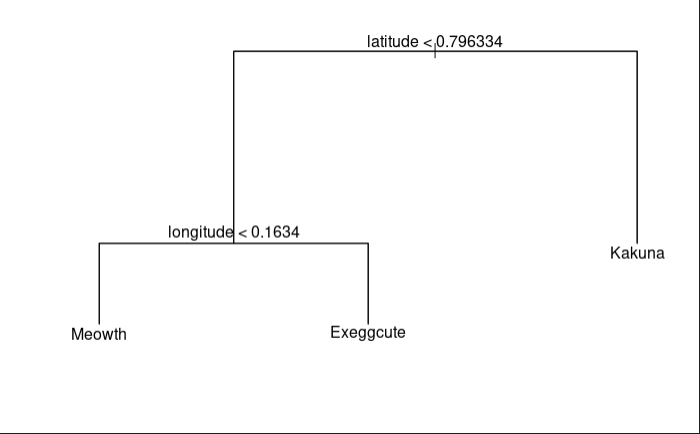
\includegraphics[width=\textwidth]{img/tree.png}
	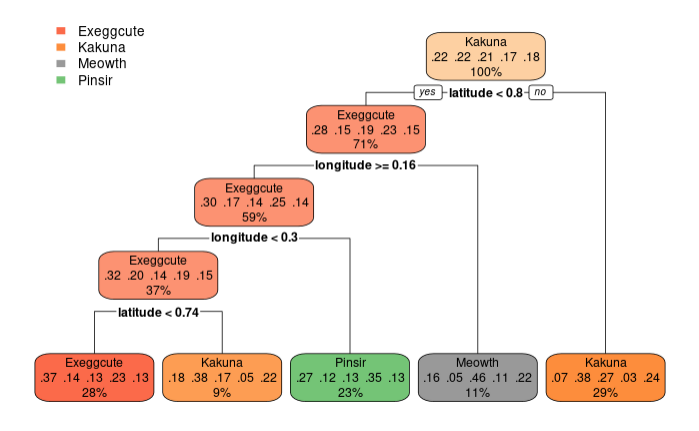
\includegraphics[width=\textwidth]{img/rpart.png}
\end{figure}

En las capturas anteriores podemos ver cómo los atributos empleados por dos de los 3 árboles de decisión construidos son \textbf{latitude} y \textbf{longitude}, de hecho observaremos esta tendencia en otro algoritmo más adelante. Pese a que rpart consigue una partición de los elementos del conjunto de train dando lugar a al menos un nodo hoja para cada una de las especies de pokemon que tenemos, no obtenemos un buen resultado de clasificación en test.\\

Para knn empleamos k = 9 ya que en una ejecución de la función \code{tune.knn} (probablemente sobre un dataset distinto al que finalmente empleamos en clasificación) obtuvimos que le mejor k precisamente 9. Si ejecutamos esta función sobre el conjunto actual obtenemos que el mejor k es 1, indicando posiblemente que las distintas clases están muy solapadas unas con otras en el dataset. Si bien es cierto que con k igual a 9 obtenemos un resultado ligeramente superior a emplear k = 1 (32.72\%).\\

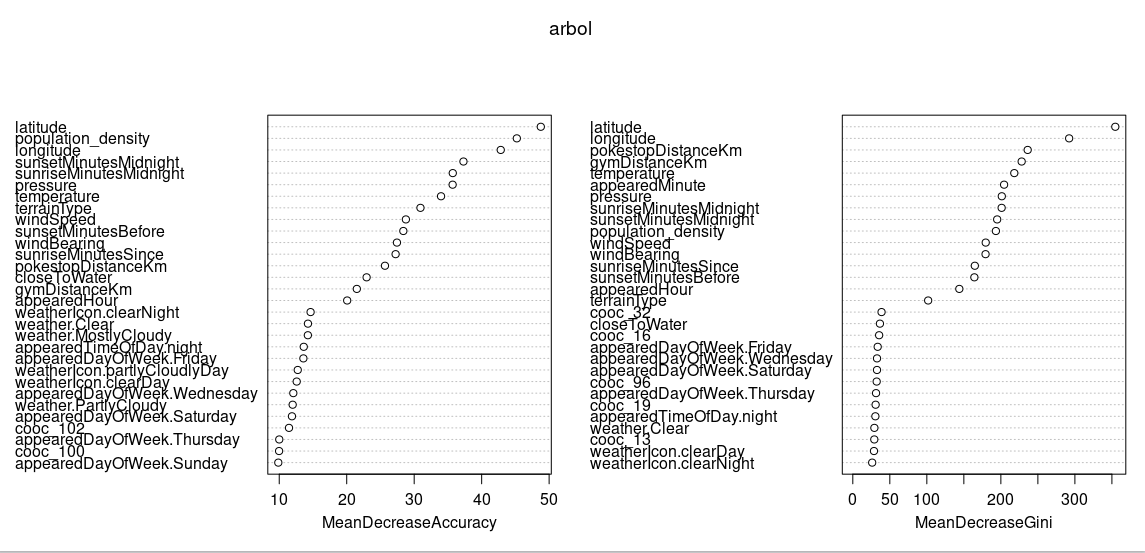
\includegraphics[width=\textwidth]{img/importancia.png}

En la gráfica anterior podemos ver cómo la longitud y la latitud vuelven a ser atributos muy determinantes para la clasificacion de los árboles de random forest, pese a que no se han obtenido tampoco unos resultados buenos en la clasificación. Tratamos, dado que estos atributos parecían tan importantes, a imponer a xgboost que sólo pudiese obtener árboles con un máximo de profundidad 2 para forzarlo a sólo usar estos dos atributos, los resultados empeoraron (ya hemos visto cómo se producen árboles de decisión más profundos usando sólo estos dos atributos en rpart).\\
 
Acabamos este estudio sobre los resultados de clasificación obtenidos haciendo una observación propia que probablemente sea errónea pero no obstante consideramos que es interesante incluirla en nuestro trabajo: el error que se puede producir en la clasificación se puede descomponer en dos componentes, el bias (la diferencia que hay entre el valor real a predecir y el predicho) y la varianza (erro debido al propio ruido del dataset). Encontrar un algoritmo que minimice ambos tipo de error simultáneamente es muy complicado y cada uno de los dos algoritmos de \textit{ensamble} que hemos empleado se centran en reducir uno de los dos. Mientras que random forest combina árboles más complejos independiente unos de otros para reducir el bias, xgboost emplea árboles más simples (aunque nosotros podemos controlar la profundidad máxima de los árboles empleados) tratando así de reducir la varianza.\\

Entonces, dado que ninguno de los dos enfoques anteriores da un resultado mucho mejor que el otro, pensamos que el dataset puede que no tenga información errónea o con ruido, pero que en cambio esta información no parece ser suficiente o adecuada para poder realizar una buena clasificación.